\def\linkdethi{} %Đường link cần dẫn tới
\anmaQR
%%%%%%%%%%%%%%%%%%%%%%%%
\def\toanlop{12}
\def\thoigian{90}
\def\namhoc{2025 - 2026}
\begin{dethi}
	{Bộ GD\&ĐT}
	{VTED ft KING EDU}
	{TDMT06}
	{Đề thi thử THPTQG 2026}
\end{dethi}
\caulc
\Opensolutionfile{ans}[ans/ansTN-Dung]
%%%=============EX_1=============%%%
\begin{ex}%[1D1H5-3]%[TDMT06]%[Đình Nguyên]
	Nghiệm của phương trình $\sin\left(x-\dfrac{\pi}{3}\right)=1$ là
	\choice
	{$x=\dfrac{5\pi}{6}+k2\pi$, $k \in \mathbb{N}$}
	{\True $x=\dfrac{5\pi}{6}+k2\pi$, $k \in \mathbb{Z}$}
	{$x=\dfrac{\pi}{2}+k2\pi$, $k \in \mathbb{Z}$}
	{$x=\dfrac{5\pi}{6}+k\pi$, $k \in \mathbb{Z}$}
	\loigiai{
		Ta có
		\begin{eqnarray*}
			&&\sin\left(x-\dfrac{\pi}{3}\right)=1\\
			&\Leftrightarrow&x - \dfrac{\pi}{3} = \dfrac{\pi}{2} + k2\pi \\
			&\Leftrightarrow& x = \dfrac{\pi}{2} + \dfrac{\pi}{3} + k2\pi \\
			&\Leftrightarrow& x= \dfrac{5\pi}{6} + k2\pi,\, (k\in\mathbb Z).
		\end{eqnarray*}
	}
\end{ex}
%%%=============================%%%

%%%=============EX_2=============%%%
\begin{ex}%[1D6N4-4]%[TDMT06]%[Nguyễn Văn Sang]
	Nghiệm của phương trình $8^x = 16$ là
	\choice
	{$\{\pm3\}$}
	{$\{2\}$}
	{$\{4\}$}
	{\True $\left\lbrace\dfrac{4}{3}\right\rbrace$}
	\loigiai{
		Ta có $8^x = 16 \Leftrightarrow 2^{3x} = 2^4 \Leftrightarrow 3x = 4 \Leftrightarrow x = \dfrac{4}{3}$.
	}
\end{ex}
%%%=============================%%%

%%%=============EX_3=============%%%
\begin{ex}%[1D2N2-4]%[TDM-Đề 6]%[Đoàn Văn Mùi]
	Cho cấp số cộng $(u_n)$ có số hạng đầu bằng $2$ và công sai bằng $3$. Số hạng $u_4$ bằng
	\choice
	{\True $11$}
	{$14$}
	{$54$}
	{$6$}
	\loigiai{
		Công thức số hạng tổng quát $u_n = u_1 + (n-1)d$.\\ Suy ra $u_4=2+3d=2+3\cdot 3=11$.
	}
\end{ex}
%%%=============================%%%

%%%=============EX_4=============%%%
\begin{ex}%[0D8N2-7]%[TDMT06]%[Nguyễn Trí Minh Tuấn]
	Số cách xếp $2$ người vào $6$ vị trí ghế hàng ngang là
	\choice
	{$\mathrm{C}_6^2$}
	{$12$}
	{\True$\mathrm{A}_6^2$}
	{$6$}
	\loigiai{
		Xếp $2$ người vào $6$ vị trí (có phân biệt thứ tự người và vị trí) là chỉnh hợp chập $2$ của $6$.\\
		Số cách là $\mathrm{A}_6^2 = 30$.
	}
\end{ex}
%%%=============================%%%

%%%=============EX_5=============%%%
\begin{ex}%[1D6H4-2]%[TDMT06]%[Trần Văn Thiện]
	Số nghiệm thực của phương trình $\log_x x^2 = \log_x 1$ là
	\choice
	{\True $0$}
	{$1$}
	{$2$}
	{$3$}
	\loigiai{
		Điều kiện $0 < x \neq 1$.\\
		Khi đó	$\log_x x^2 = \log_x 1$ trở thành $x^2=1$ $\Leftrightarrow x = \pm 1$.\\
		Đối chiếu điều kiện $0 < x \neq 1$, không có giá trị nào thỏa mãn.\\
		Vậy phương trình vô nghiệm.
	}
\end{ex}
%%%=============================%%%

%%%=============EX_6=============%%%
\begin{ex}%[1H8H7-2]%[TDMT06]%[Phạm Hải Dương]
	Cho hình chóp $S. ABC$ có đáy là tam giác vuông cân có cạnh huyền bằng $3\sqrt{2}$, cạnh bên $SA$ vuông góc với đáy và $SA=2$. Thể tích của khối chóp $S. ABC$ là
	\choice
	{$6$}
	{\True $3$}
	{$4$}
	{$12$}
	\loigiai{
		\immini{Tam giác $ABC$ vuông cân có cạnh huyền bằng $3\sqrt{2}$ nên suy ra cạnh góc vuông bằng $3$.\\
			Diện tích đáy $S_{ABC} = \dfrac{1}{2} \cdot 3 \cdot 3 = 4{,}5$.\\
			Thể tích $V = \dfrac{1}{3} \cdot S_{ABC} \cdot SA = \dfrac{1}{3} \cdot 4{,}5 \cdot 2 = 3$.}{\begin{tikzpicture}[>=stealth,line join=round,line cap=round,font=\footnotesize,scale=1]
				\def\ha{2} \def\ca{1.5} \def\cb{2}
				\path
				(0,0)coordinate(A)
				($(A)+(0,\ha)$)coordinate(S)
				(-40:\ca)coordinate(C)
				(\cb,0)coordinate(B)
				;
				\draw(S)--(A)--(C)--(B)--cycle
				(S)--(C)
				;
				\draw[dashed](A)--(B);
				\foreach \x/\g in {A/150,S/0,C/-90,B/0}\fill[black](\x)circle(1pt)+(\g:.3)node{$\x$};
		\end{tikzpicture}}
	}
\end{ex}
%%%=============================%%%

%%%=============EX_7=============%%%
\begin{ex}%[2D1N2-2]%[TDMT06]%[Văn Minh Thoại]
	\immini[thm]{
		Cho đồ thị hàm số $y=f(x)$ như hình vẽ bên. Cực tiểu của hàm số $f(x)$ là
		\choice[1]
		{$3$}
		{$4$}
		{\True $0$}
		{$-1$}
	}{
		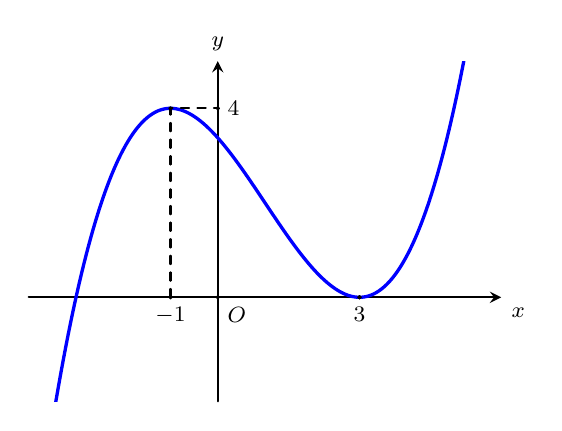
\begin{tikzpicture}[font=\footnotesize,line join=round,line cap=round,>=stealth,scale=0.6]
			\def \xmin{-4}
			\def \xmax{6}
			\def \ymin{-2.2}
			\def \ymax{5}
			\draw[->,thick] (\xmin,0) -- (\xmax,0) node[below right] {$x$};
			\draw[->,thick] (0,\ymin) -- (0,\ymax) node[above] {$y$};
			\clip (\xmin,\ymin) rectangle (\xmax,\ymax);
			\draw[blue,very thick]
			plot[domain=\xmin:\xmax,samples=500]
			(\x,{((\x*\x*\x) - 3*(\x*\x) - 9*\x + 27)/8});
			\draw[dashed,thick] (-1,0) |- (0,4);
			\foreach \P in {(-1,0),(0,0),(3,0),(0,4),(-1,4),(3,0)}{
				\filldraw[fill=black,draw=black] \P circle (1pt);	}
			\node[below] at (-1,0) {$-1$};
			\node[below] at (3,0) {$3$};
			\node[right] at (0,4) {$4$};
			\node[below right] at (0,0) {$O$};
		\end{tikzpicture}
	}
	\loigiai{
		Dựa vào đồ thị, hàm số đạt cực tiểu tại điểm $x=3$ và giá trị cực tiểu tương ứng là $y_{\text{CT}}=0$.
	}
\end{ex}
%%%=============================%%%

%%%=============EX_8=============%%%
\begin{ex}%[2D1H4-1]%[TDMT06]%[Lê Phúc]
	Tiệm cận xiên của đồ thị hàm số $y = \dfrac{x^2-2x-4}{x+1}$ là
	\choice
	{$y=x+1$}
	{$x=-1$}
	{$y=x$}
	{\True $y=x-3$}
	\loigiai{
		Thực hiện phép chia đa thức ta có $y = \dfrac{x^2-2x-4}{x+1}=x-3-\dfrac{1}{x+1}$.\\
		Suy ra $\lim\limits_{x\rightarrow \pm\infty}\left[y-(x-3)\right]=\lim\limits_{x\rightarrow \pm\infty}\left(-\dfrac{1}{x+1}\right)=0$.\\
		Vậy tiệm cận xiên của đồ thị hàm số là $y = x - 3$.
	}
\end{ex}
%%%=============================%%%

%%%=============EX_9=============%%%
\begin{ex}%[2D1H2-1]%[TDMT06]%[Vũ Hồng Toàn]
	Hàm số $y = -x^3 + 3x^2 + 2\,026$ có điểm cực đại là
	\choice
	{\True $x=2$}
	{$x=0$}
	{$y=2\,026$}
	{$y=2\,030$}
	\loigiai{
		Tập xác định $\mathscr{D}=\mathbb{R}$.\\
		Ta có $y = -x^3 + 3x^2 + 2\,026\Rightarrow y' = -3x^2 + 6x$.\\
		Cho $y'=0 \Leftrightarrow x=0$ hoặc $x=2$.\\
		Bảng biến thiên
		\begin{center}
			
\begin{tikzpicture}
				\tkzTabInit[nocadre=false, lgt=1, espcl=3, deltacl=0.5]
				{$x$/0.7,$y'$/0.7,$y$/2}
				{$-\infty$,$0$,$2$,$+\infty$}
				\tkzTabLine{,-,0,+,0,-,}
				\tkzTabVar{+/$+\infty$,-/$2\,026$,+/$2\,030$,-/$-\infty$}
			\end{tikzpicture}
		\end{center}
		Quan sát bảng biến thiên ta nhận thấy hàm số đạt cực tiểu tại $x=0$ và cực đại tại $x=2$.
	}
\end{ex}
%%%=============================%%%

%%%=============EX_10=============%%%
\begin{ex}%%[2D1H3-1]%[TDMT06]%[Chu Ha]
	\immini[thm]
	{
		Cho bảng biến thiên của hàm số $y=f(x)$ như hình vẽ bên. \\
		Giá trị lớn nhất của hàm số $y=f(x)$ trên đoạn $[-3; 1]$ bằng
		\choice
		{$0$}
		{\True $6$}
		{$-5$}
		{$2$}
	}
	{
		
\begin{tikzpicture}
			\tkzTabInit[nocadre=false,lgt=1.2,espcl=1.8]{$x$/0.8,$f(x)$/2}
			{$-\infty$,$-5$,$0$,$2$,$+\infty$}
			\tkzTabVar{+/$+\infty$,-/$-1$,+/$6$,-/$2$,+/$+\infty$}
		\end{tikzpicture}
		
	}
	\loigiai{
		Trên đoạn $[-3; 1]$, hàm số tăng lên đến giá trị cực đại là $6$ tại $x=0$ rồi giảm xuống.\\
		Giá trị lớn nhất của hàm số $y=f(x)$ trên đoạn $[-3; 1]$ bằng $6$.
	}
\end{ex}
%%%=============================%%%

%%%=============EX_11=============%%%
\begin{ex}
	\sochc{2}
	\immini{Cho hình chóp tứ giác đều $S.ABCD$ có cạnh đáy bằng $4$ và cạnh bên bằng $6$. Gọi $O$ là tâm của đáy.}
	{
		\begin{tikzpicture}[declare function={a=2.5; b=4; h=4; goc=-140;}, line join=round, line cap=round, >=stealth, font=\footnotesize, scale=0.8]
			\path
			(0,0) coordinate (A)
			(b,0) coordinate (D)
			(goc:a) coordinate (B)
			($(B)+(D)$) coordinate (C)
			($(B)!0.5!(D)$) coordinate (O)
			($(O)+(0,h)$) coordinate (S);
			
			\draw[dashed] (B)--(A)--(D) (S)--(A) (S)--(O) (A)--(C) (B)--(D);
			\draw (B)--(C)--(D) (S)--(B) (S)--(C) (S)--(D);
			
			\foreach \x/\g in {S/90, A/135, B/-135, C/-45, D/0, O/-90}
			\filldraw (\x) circle (1pt) node[shift={(\g:3mm)}]{$\x$};
		\end{tikzpicture}
	}
	
	%%%=============CHC_1=============%%%
	\begin{chc}%[2H2N1-2]%[TDMT06]%[Đỗ Đường Hiếu]
		Tổng $\overrightarrow{SA}+\overrightarrow{SB}+\overrightarrow{SC}+\overrightarrow{SD}$ bằng
		\choice
		{$2\overrightarrow{SO}$}
		{$\overrightarrow{SO}$}
		{$\overrightarrow{0}$}
		{\True $4\overrightarrow{SO}$}
		\loigiai{
			Vì $O$ là trung điểm của $AC$ và $BD$ nên
			\[\heva{&\overrightarrow{SA}+\overrightarrow{SC} = 2\overrightarrow{SO}\\&\overrightarrow{SB}+\overrightarrow{SD}= 2\overrightarrow{SO}}\Rightarrow \overrightarrow{SA}+\overrightarrow{SB}+\overrightarrow{SC}+\overrightarrow{SD}=4\overrightarrow{SO}.\]
		}
	\end{chc}
	%%%=============================%%%
	
	%%%=============CHC_2=============%%%
	\begin{chc}%[2H2H1-3]%[TDMT06]%[Đỗ Đường Hiếu]
		Giá trị của biểu thức $\left(\overrightarrow{SB} - \overrightarrow{SC}\right)\overrightarrow{SD}$ bằng
		\choice
		{\True $-8$}
		{$8$}
		{$12$}
		{$-12$}
		\loigiai{
			Ta có
			\allowdisplaybreaks
			\begin{align*}
				\left(\overrightarrow{SB} - \overrightarrow{SC}\right)\overrightarrow{SD} &= \overrightarrow{CB}\cdot \left(\overrightarrow{OD}-\overrightarrow{OS}\right) \\
				&=\left(\overrightarrow{OB}-\overrightarrow{OC}\right)\cdot \left(-\overrightarrow{OB}-\overrightarrow{OS}\right)\\
				&=-\overrightarrow{OB}^2-\overrightarrow{OB}\cdot\overrightarrow{OS}+\overrightarrow{OC}\cdot \overrightarrow{OD}+\overrightarrow{OC}\cdot \overrightarrow{OS}\\
				&=-OB^2=-\left(\dfrac{BD}{2}\right)^2=-\left(\dfrac{4\sqrt{2}}{2}\right)^2 =-8.
			\end{align*}
		}
	\end{chc}
	%%%=============================%%%
\end{ex}
%%%=============================%%%
\Closesolutionfile{ans}

\cauds
\Opensolutionfile{ans}[ans/ansTN-DungSai]
%%%=============EX_13=============%%%
\begin{ex}%[2D1V3-2]%[TDMT06]%[Huỳnh Quốc Đạt]
	Cho hàm số $y=f(x)=\mathrm{e}^x - \ln(x+1)$.
	\choiceTF[t]
	{$f'(x) = \mathrm{e}^x + \dfrac{1}{x+1}$, $\forall x > -1$}
	{\True $f'(0)=0$}
	{\True Hàm số $f'(x)$ đồng biến trên khoảng $(-1; +\infty)$}
	{\True $\min f(x) = 1$}
	\loigiai{
		\begin{itemchoice}
			\itemch
			Tập xác định $\mathscr{D}=(-1;+\infty)$.\\
			$f'(x) = \mathrm{e}^x - \dfrac{1}{x+1}$.
			\itemch $f'(0) = \mathrm{e}^0 - \dfrac{1}{1} = 0$.
			\itemch $f''(x) = \mathrm{e}^x + \dfrac{1}{(x+1)^2} > 0$, $\forall x>-1$ nên $f'(x)$ đồng biến trên $(-1;+\infty)$.
			\itemch Ta có $f'(x) = \mathrm{e}^x - \dfrac{1}{x+1}$.\\
			Vì hàm số $f'(x)$ đồng biến trên $(-1;+\infty)$ (theo câu c) và $f'(0)=0$ nên phương trình $f'(x)=0$ có nghiệm duy nhất $x=0$.\\
			Bảng biến thiên
			\begin{center}
				
\begin{tikzpicture}
					\tkzTabInit[lgt=1.2,espcl=2.5,nocadre=false]
					{$x$/0.7,$f(x)$/2}
					{$-1$, $0$,$+\infty$}
					\tkzTabVar{+/$+\infty$, -/$1$, +/$+\infty$}
				\end{tikzpicture}
			\end{center}
			Dựa vào bảng biến thiên ta có $\min f(x) = 1$.
		\end{itemchoice}
	}
\end{ex}
%%%=============================%%%

%%%=============EX_14=============%%%
\begin{ex}%[2D1H3-6]%[ID]%[TDMT06]%[Dương Công Tạo]
	Doanh thu từ việc thuê $x$ căn hộ có thể được mô hình hoá bằng hàm số \[R(x)=2x\left(900+32x-x^2\right)\text{ (USD), với } 0<x<50.\]
	\choiceTF[t]
	{Hàm doanh thu biên là $R'(x) = -4x^2 + 64x + 1\,800$ USD/ căn hộ}
	{\True Doanh thu biên khi $x=12$ là $2\,472$ USD/ căn hộ}
	{Lượng doanh thu tăng thêm $2\,472$ USD khi số căn hộ cho thuê tăng từ $12$ lên $13$ căn hộ}
	{\True Doanh thu bình quân lớn nhất bằng $2\,312$ USD/ căn hộ}
	\loigiai{
		\begin{itemchoice}
			\itemch Ta có $R(x)=2x\left(900+32x-x^2\right)= 1\,800x + 64x^2 - 2x^3$.\\
			Khi đó, hàm doanh thu biên là $R'(x) = 1\,800 + 128x - 6x^2$ USD/ căn hộ.
			\itemch Doanh thu biên khi $x=12$ là $R'(12) = 1\,800 + 128\cdot 12 - 6\cdot 12^2 = 2\,472$.
			\itemch Lượng doanh thu tăng thêm thực tế là $\Delta R = R(13) - R(12) = 2\,462$ USD (khác $2\,472$). Giá trị đạo hàm chỉ là xấp xỉ lượng tăng.
			\itemch Doanh thu bình quân $\overline{R}(x) = \dfrac{R(x)}{x} = 1\,800 + 64x - 2x^2=-2(x-16)^2+2\,312\leq 2\,312$. \\
			Vậy, doanh thu bình quân lớn nhất bằng $2\,312$ USD/ căn hộ khi cho thuê $16$ căn hộ.
		\end{itemchoice}
	}
\end{ex}
%%%=============================%%%

%%%=============EX_15=============%%%
\begin{ex}%[2H2V1-4]%[TDMT06]%[Nguyễn Tấn Linh]
	Trong không gian cho ba sợi dây có khối lượng không đáng kể được buộc chung một đầu $A$ và được kéo căng về ba hướng bởi ba lực $\overrightarrow{F}_1$, $\overrightarrow{F}_2$, $\overrightarrow{F}_3$ như hình vẽ. Biết rằng các lực kéo làm ba sợi dây ở trạng thái đứng yên. Cho $\left|\overrightarrow{F}_1\right|=60$\,N, $\left(\overrightarrow{F}_2,\overrightarrow{F}_3\right)=60^{\circ}$.
	\begin{center}
		\definecolor{ropeColor}{HTML}{CDB38B}
		\definecolor{outlineColor}{HTML}{4A2E19}
		\definecolor{highlightColor}{HTML}{E8DCC5} 
		\definecolor{forceColor}{HTML}{B03A2E} 
		\begin{tikzpicture}[scale=1,>=stealth]
			\begin{scope}[
				color=ropeColor,
				line width=3.2pt,
				line cap=round,
				postaction={
					draw,
					color=highlightColor,
					line width=1.2pt,
					line cap=round,
					opacity=0.6, 
					shorten >=0.5pt,
					shorten <=0.5pt
				}
				]
				\draw (1.33,1.46) .. controls +(31.0:0.18) and +(164.1:0.22) .. (1.85,1.48);
				\draw (1.74,1.51) .. controls +(35.0:0.18) and +(153.4:0.24) .. (2.30,1.58);
				\draw (2.12,1.63) .. controls +(32.5:0.20) and +(160.3:0.23) .. (2.64,1.68);
				\draw (2.55,1.71) .. controls +(38.7:0.29) and +(153.4:0.24) .. (3.15,1.73);
				\draw (2.95,1.81) .. controls +(21.8:0.16) and +(161.6:0.24) .. (3.50,1.83);
				\draw (3.33,1.87) .. controls +(19.7:0.23) and +(161.6:0.14) .. (3.85,1.94);
				\draw (3.71,1.96) .. controls +(38.7:0.19) and +(159.8:0.31) .. (4.38,2.08);
				\draw (4.20,2.12) .. controls +(42.5:0.25) and +(146.9:0.42) .. (4.94,2.14);
				\draw (4.58,2.28) .. controls +(91.6:0.53) and +(153.4:0.34) .. (5.41,2.58);
				\draw (4.80,2.67) .. controls +(76.0:0.37) and +(118.9:0.50) .. (5.70,2.61);
				\draw (5.20,2.94) .. controls +(42.9:0.58) and +(86.2:0.46) .. (5.97,2.52);
				\draw (5.77,3.05) .. controls +(1.6:0.55) and +(65.2:0.43) .. (6.17,2.29);
				\draw (6.23,2.86) .. controls +(-15.9:0.44) and +(61.2:0.35) .. (6.41,2.14);
				\draw (6.53,2.44) .. controls +(-68.2:0.16) and +(58.0:0.14) .. (6.53,2.1);
				\draw (5.86,2.2) .. controls +(52.4:0.25) and +(64.1:0.59) .. (5.35,2.39);
				\draw (5.14,2.03) .. controls +(79.7:0.34) and +(166.0:0.44) .. (5.85,2.44);
				\draw (5.00,1.77) .. controls +(76.8:0.26) and +(-177.1:0.30) .. (5.59,2.15);
				\draw (4.85,1.74) .. controls +(-106.6:0.58) and +(-93.9:0.67) .. (5.67,1.9);
				\draw (4.97,1.74) .. controls +(-24.2:0.33) and +(-111.8:0.49) .. (5.85,2.19);
				\draw (5.36,1.41) .. controls +(-122.6:0.45) and +(-111.8:0.65) .. (4.65,1.68);
				\draw (5.9,2.2) .. controls +(180.0:0.18) and +(37.9:0.17) .. (5.36,2);
				\draw (5.00,1.82) .. controls +(161.6:0.24) and +(-33.7:0.16) .. (4.52,2.06);
				\draw (4.91,1.85) .. controls +(-126.0:0.41) and +(-20.6:0.39) .. (4.02,1.88);
				\draw (4.45,1.7) .. controls +(-143.1:0.38) and +(-28.3:0.22) .. (3.68,1.76);
				\draw (4.03,1.6) .. controls +(-138.8:0.32) and +(-30.1:0.33) .. (3.26,1.68);
				\draw (3.64,1.5) .. controls +(-126.4:0.36) and +(-23.2:0.35) .. (2.82,1.61);
				\draw (3.24,1.4) .. controls +(-136.8:0.33) and +(-33.7:0.27) .. (2.55,1.48);
				\draw (2.88,1.3) .. controls +(-144.8:0.32) and +(-21.3:0.29) .. (2.11,1.36);
				\draw (2.47,1.23) .. controls +(-139.4:0.28) and +(-25.5:0.35) .. (1.70,1.27);
				\draw (2.09,1.13) .. controls +(-150.9:0.31) and +(-26.6:0.20) .. (1.33,1.12)--(1.33,1.46);
				\draw (5.9,2.2) .. controls +(0.0:0.18) and +(111.3:0.29) .. (6.42,1.86);
				\draw (6.2,2.13) .. controls +(7.4:0.4) and +(135.0:0.19) .. (6.74,1.89);
				\draw (6.64,2) .. controls +(14.0:0.19) and +(120.5:0.30) .. (7.17,1.86);
				\draw (7.05,2.00) .. controls +(14.0:0.19) and +(142.4:0.25) .. (7.59,1.83);
				\draw (7.48,1.9) .. controls +(0.0:0.18) and +(135.0:0.17) .. (8.00,1.79);
				\draw (7.88,1.87) .. controls +(4.8:0.18) and +(131.2:0.16) .. (8.32,1.74) .. controls +(29.7:0.24) and +(155.2:0.22) .. (8.83,1.68);
				\draw (8.83,1.68)--(8.83,1.17) .. controls +(148.4:0.23) and +(-56.3:0.22) .. (8.44,1.62);
				\draw (8.74,1.24) .. controls +(-166.0:0.19) and +(-34.7:0.24) .. (8.20,1.39);
				\draw (8.32,1.32) .. controls +(-144.0:0.21) and +(-74.1:0.44) .. (7.67,1.74);
				\draw (7.91,1.36) .. controls +(-172.9:0.24) and +(-52.6:0.32) .. (7.29,1.68);
				\draw (7.48,1.47) .. controls +(-167.0:0.20) and +(-60.0:0.45) .. (6.79,1.83);
				\draw (7.14,1.49) .. controls +(-172.2:0.34) and +(-48.0:0.20) .. (6.52,1.77);
				\draw (6.76,1.55) .. controls +(-177.3:0.32) and +(-45.0:0.19) .. (6.15,1.77);
				\draw (6.32,1.63) .. controls +(-165.3:0.30) and +(-60.3:0.24) .. (5.76,1.85);
				\draw (6.35,1.62) .. controls +(-112.4:0.28) and +(-47.7:0.23) .. (5.79,1.61);
				\draw (6.09,1.46) .. controls +(-113.2:0.23) and +(-83.4:0.40) .. (5.59,1.64);
				\draw (5.8,1.33) .. controls +(-158.2:0.3) and +(-53.1:0.15) .. (5.35,1.41);
				\draw (5.15,2.94) .. controls +(97.1:0.24) and +(0.0:0.36) .. (4.83,3.44);
				\draw (4.82,3.21) .. controls +(70.0:0.18) and +(-37.9:0.17) .. (4.7,3.64);
				\draw (4.67,3.4) .. controls +(63.4:0.14) and +(-41.6:0.4) .. (4.46,3.94);
				\draw (4.42,3.83) .. controls +(59.7:0.21) and +(-37.9:0.17) .. (4.30,4.35);
				\draw (4.6,2.47) .. controls +(105.5:0.28) and +(-136.8:0.33) .. (4.71,3.15);
				\draw (4.55,2.65) .. controls +(135.0:0.26) and +(-129.0:0.41) .. (4.52,3.41);
				\draw (4.37,3.00) .. controls +(144.5:0.26) and +(-140.4:0.45) .. (4.42,3.79);
				\draw (4.19,3.33) .. controls +(128.7:0.19) and +(-127.4:0.32) .. (4.15,4.05);
				\draw (4.05,3.62) .. controls +(147.3:0.25) and +(-126.4:0.36) .. (3.94,4.35)--(4.30,4.35);
			\end{scope}
			\begin{scope}[color=outlineColor]
				\draw [line width=0.3pt] (1.33,1.46)
				.. controls +(31.0:0.18) and +(164.1:0.22) .. (1.85,1.48);
				\draw [line width=0.3pt] (1.74,1.51)
				.. controls +(35.0:0.18) and +(153.4:0.24) .. (2.30,1.58);
				\draw [line width=0.3pt] (2.12,1.63)
				.. controls +(32.5:0.20) and +(160.3:0.23) .. (2.64,1.68);
				\draw [line width=0.3pt] (2.55,1.71)
				.. controls +(38.7:0.29) and +(153.4:0.24) .. (3.15,1.73);
				\draw [line width=0.3pt] (2.95,1.81)
				.. controls +(21.8:0.16) and +(161.6:0.24) .. (3.50,1.83);
				\draw [line width=0.3pt] (3.33,1.87)
				.. controls +(19.7:0.23) and +(161.6:0.14) .. (3.85,1.94);
				\draw [line width=0.3pt] (3.71,1.96)
				.. controls +(38.7:0.19) and +(159.8:0.31) .. (4.38,2.08);
				\draw [line width=0.3pt] (4.20,2.12)
				.. controls +(42.5:0.25) and +(146.9:0.42) .. (4.94,2.14);
				\draw [line width=0.3pt] (4.58,2.28)
				.. controls +(91.6:0.53) and +(153.4:0.34) .. (5.41,2.58);
				\draw [line width=0.3pt] (4.80,2.67)
				.. controls +(76.0:0.37) and +(118.9:0.50) .. (5.70,2.61);
				\draw [line width=0.3pt] (5.20,2.94)
				.. controls +(42.9:0.58) and +(86.2:0.46) .. (5.97,2.52);
				\draw [line width=0.3pt] (5.77,3.05)
				.. controls +(1.6:0.55) and +(65.2:0.43) .. (6.17,2.29);
				\draw [line width=0.3pt] (6.23,2.86)
				.. controls +(-15.9:0.44) and +(61.2:0.35) .. (6.41,2.14);
				\draw [line width=0.3pt] (6.53,2.44)
				.. controls +(-68.2:0.16) and +(58.0:0.14) .. (6.53,2.1);
				\draw [line width=0.3pt] (5.86,2.2)
				.. controls +(52.4:0.25) and +(64.1:0.59) .. (5.35,2.39);
				\draw [line width=0.3pt] (5.14,2.03)
				.. controls +(79.7:0.34) and +(166.0:0.44) .. (5.85,2.44);
				\draw [line width=0.3pt] (5.00,1.77)
				.. controls +(76.8:0.26) and +(-177.1:0.30) .. (5.59,2.15);
				\draw [line width=0.3pt] (4.85,1.74)
				.. controls +(-106.6:0.58) and +(-93.9:0.67) .. (5.67,1.9);
				\draw [line width=0.3pt] (4.97,1.74)
				.. controls +(-24.2:0.33) and +(-111.8:0.49) .. (5.85,2.19);
				\draw [line width=0.3pt] (5.36,1.41)
				.. controls +(-122.6:0.45) and +(-111.8:0.65) .. (4.65,1.68);
				\draw [line width=0.3pt] (5.9,2.2)
				.. controls +(180.0:0.18) and +(37.9:0.17) .. (5.36,2);
				\draw [line width=0.3pt] (5.00,1.82)
				.. controls +(161.6:0.24) and +(-33.7:0.16) .. (4.52,2.06);
				\draw [line width=0.3pt] (4.91,1.85)
				.. controls +(-126.0:0.41) and +(-20.6:0.39) .. (4.02,1.88);
				\draw [line width=0.3pt] (4.45,1.7)
				.. controls +(-143.1:0.38) and +(-28.3:0.22) .. (3.68,1.76);
				\draw [line width=0.3pt] (4.03,1.6)
				.. controls +(-138.8:0.32) and +(-30.1:0.33) .. (3.26,1.68);
				\draw [line width=0.3pt] (3.64,1.5)
				.. controls +(-126.4:0.36) and +(-23.2:0.35) .. (2.82,1.61);
				\draw [line width=0.3pt] (3.24,1.4)
				.. controls +(-136.8:0.33) and +(-33.7:0.27) .. (2.55,1.48);
				\draw [line width=0.3pt] (2.88,1.3)
				.. controls +(-144.8:0.32) and +(-21.3:0.29) .. (2.11,1.36);
				\draw [line width=0.3pt] (2.47,1.23)
				.. controls +(-139.4:0.28) and +(-25.5:0.35) .. (1.70,1.27);
				\draw [line width=0.3pt] (2.09,1.13)
				.. controls +(-150.9:0.31) and +(-26.6:0.20) .. (1.33,1.12)--(1.33,1.46);
				\draw (5.9,2.2) .. controls +(0.0:0.18) and +(111.3:0.29) .. (6.42,1.86);
				\draw (6.2,2.13) .. controls +(7.4:0.4) and +(135.0:0.19) .. (6.74,1.89);
				\draw (6.64,2) .. controls +(14.0:0.19) and +(120.5:0.30) .. (7.17,1.86);
				\draw (7.05,2.00) .. controls +(14.0:0.19) and +(142.4:0.25) .. (7.59,1.83);
				\draw (7.48,1.9) .. controls +(0.0:0.18) and +(135.0:0.17) .. (8.00,1.79);
				\draw (7.88,1.87) .. controls +(4.8:0.18) and +(131.2:0.16) .. (8.32,1.74) .. controls +(29.7:0.24) and +(155.2:0.22) .. (8.83,1.68);
				\draw (8.83,1.68)--(8.83,1.17) .. controls +(148.4:0.23) and +(-56.3:0.22) .. (8.44,1.62);
				\draw (8.74,1.24) .. controls +(-166.0:0.19) and +(-34.7:0.24) .. (8.20,1.39);
				\draw (8.32,1.32) .. controls +(-144.0:0.21) and +(-74.1:0.44) .. (7.67,1.74);
				\draw (7.91,1.36) .. controls +(-172.9:0.24) and +(-52.6:0.32) .. (7.29,1.68);
				\draw (7.48,1.47) .. controls +(-167.0:0.20) and +(-60.0:0.45) .. (6.79,1.83);
				\draw (7.14,1.49) .. controls +(-172.2:0.34) and +(-48.0:0.20) .. (6.52,1.77);
				\draw (6.76,1.55) .. controls +(-177.3:0.32) and +(-45.0:0.19) .. (6.15,1.77);
				\draw (6.32,1.63) .. controls +(-165.3:0.30) and +(-60.3:0.24) .. (5.76,1.85);
				\draw (6.35,1.62) .. controls +(-112.4:0.28) and +(-47.7:0.23) .. (5.79,1.61);
				\draw (6.09,1.46) .. controls +(-113.2:0.23) and +(-83.4:0.40) .. (5.59,1.64);
				\draw (5.8,1.33) .. controls +(-158.2:0.3) and +(-53.1:0.15) .. (5.35,1.41);
				\draw (5.15,2.94) .. controls +(97.1:0.24) and +(0.0:0.36) .. (4.83,3.44);
				\draw (4.82,3.21) .. controls +(70.0:0.18) and +(-37.9:0.17) .. (4.7,3.64);
				\draw (4.67,3.4) .. controls +(63.4:0.14) and +(-41.6:0.4) .. (4.46,3.94);
				\draw (4.42,3.83) .. controls +(59.7:0.21) and +(-37.9:0.17) .. (4.30,4.35);
				\draw (4.6,2.47) .. controls +(105.5:0.28) and +(-136.8:0.33) .. (4.71,3.15);
				\draw (4.55,2.65) .. controls +(135.0:0.26) and +(-129.0:0.41) .. (4.52,3.41);
				\draw (4.37,3.00) .. controls +(144.5:0.26) and +(-140.4:0.45) .. (4.42,3.79);
				\draw (4.19,3.33) .. controls +(128.7:0.19) and +(-127.4:0.32) .. (4.15,4.05);
				\draw (4.05,3.62) .. controls +(147.3:0.25) and +(-126.4:0.36) .. (3.94,4.35)--(4.30,4.35);
			\end{scope}
			\tikzset{forceVector/.style={line width=2pt, color=forceColor, -{Stealth[length=3mm, width=2mm]}}}
			\draw [forceVector] (3.92,1.26) -- node[below, black]{$\overrightarrow{F}_3$}(1.61,0.53);
			\draw [forceVector] (6.85,2.5) --node[above, black]{$\overrightarrow{F}_1$} (9.23,2.2);
			\draw [forceVector] (4.03,2.85) --node[left, black]{$\overrightarrow{F}_2$} (3.2,4.3);
			\shade[ball color=gray] (5.32,1) circle (3pt);
			\node[right] at (5.32,1) {\fontsize{15pt}{0}\selectfont $A$};
		\end{tikzpicture}
	\end{center}
	\choiceTF[t]
	{\True $\overrightarrow{F}_1+\overrightarrow{F}_2+\overrightarrow{F}_3=\overrightarrow{0}$}
	{\True Ba sợi dây cùng thuộc một mặt phẳng}
	{\True Nếu $\left|\overrightarrow{F}_2\right|=40$\,N thì $\left|\overrightarrow{F}_3\right|=29$\,N (\textit{làm tròn kết quả đến hàng đơn vị})}
	{Giá trị lớn nhất của $\left|\overrightarrow{F}_3\right|$ là $52{,}5$\,N (\textit{làm tròn kết quả đến hàng phần mười})}
	\loigiai{
		\begin{itemchoice}
			\itemch Do vật đứng yên nên tổng hợp lực tác dụng lên vật bằng $\overrightarrow{0}$, tức là $\overrightarrow{F}_1+\overrightarrow{F}_2+\overrightarrow{F}_3=\overrightarrow{0}$.			
			\itemch Từ đẳng thức trên ta có $\overrightarrow{F}_1 = -\left(\overrightarrow{F}_2+\overrightarrow{F}_3\right)$. Vì vectơ tổng $\overrightarrow{F}_2+\overrightarrow{F}_3$ nằm trong mặt phẳng xác định bởi hai vectơ $\overrightarrow{F}_2$ và $\overrightarrow{F}_3$, nên vectơ $\overrightarrow{F}_1$ (cùng phương ngược chiều với vectơ tổng) cũng nằm trong mặt phẳng đó.			
			\itemch Bình phương vô hướng đẳng thức lực:
			\begin{align*}
				\overrightarrow{F}_1^2 &= \left[-\left(\overrightarrow{F}_2+\overrightarrow{F}_3\right)\right]^2 = \overrightarrow{F}_2^2 + \overrightarrow{F}_3^2 + 2\overrightarrow{F}_2 \cdot \overrightarrow{F}_3 \\
				\Rightarrow F_1^2 &= F_2^2 + F_3^2 + 2 F_2 F_3 \cos 60^{\circ}
			\end{align*}
			Thay số $60^2 = 40^2 + F_3^2 + 40 F_3 \Leftrightarrow F_3^2 + 40F_3 - 2000 = 0$.
			\\Giải phương trình bậc 2, lấy nghiệm dương: $F_3 = -20 + 20\sqrt{6} \approx 28{,}99$\,N.			
			\itemch Xét lại phương trình $F_1^2 = F_2^2 + F_3^2 + F_2F_3 \Leftrightarrow F_2^2 + F_3 \cdot F_2 + (F_3^2 - 3600) = 0$.
			\\Để tồn tại lực $F_2$ (là số thực dương), phương trình bậc hai theo ẩn $F_2$ phải có ít nhất một nghiệm dương.
			\\Nhận thấy tổng hai nghiệm $S = -F_3 < 0$, nên để có nghiệm dương thì tích hai nghiệm phải $\le 0$ (hai nghiệm trái dấu).
			\\Khi đó $P = F_3^2 - 3600 \le 0 \Leftrightarrow F_3 \le 60$.
			\\Vậy giá trị lớn nhất của $\left|\overrightarrow{F}_3\right|$ là $60\,\mathrm{N}$. 
			\\\textit{Cách hiểu hình học:} Tam giác lực có cạnh $F_1=60$ đối diện với góc tù $120^\circ$ (bù với góc $60^\circ$ giữa hai vectơ thành phần), do đó $F_1$ phải là cạnh lớn nhất.\\
			Suy ra $F_3 < F_1 = 60$.
		\end{itemchoice}
	}
\end{ex}
%%%=============================%%%

%%%=============EX_16=============%%%
\begin{ex}%[0D0V2-9]%[TDMT06]%[Nguyễn Đức Tuấn Anh]
	Cho hai hộp, ban đầu hộp I đựng $6$ viên bi đỏ và $3$ viên bi xanh, hộp II đựng $5$ viên bi đỏ và $4$ viên bi xanh.
	\begin{itemize}
		\item Hành động $1$: Lấy ngẫu nhiên $2$ viên bi từ hộp I bỏ sang hộp II.
		\item Hành động $2$: Sau đó, tiến hành lấy ngẫu nhiên $2$ viên bi từ hộp II bỏ sang hộp I.
	\end{itemize}
	\choiceTF[t]
	{\True Ở hành động $1$, có tất cả $36$ cách lấy $2$ viên bi từ hộp I sang hộp II}
	{\True Xác suất để sau hành động $1$, hộp II có $6$ bi đỏ là $0{,}5$}
	{\True Xác suất để sau hành động $2$, hộp I có $8$ viên bi đỏ là $\dfrac{1}{66}$}
	{\True Xác suất để sau hành động $2$, hộp I vẫn như ban đầu là $\dfrac{5}{11}$}
	\loigiai{
		\begin{itemchoice}
			\itemch Số cách lấy $2$ viên bi từ hộp I có $9$ viên bi là $\mathrm{C}_{9}^{2} = 36$.
			\itemch Sau hành động $1$, để hộp II có $6$ bi đỏ (tăng $1$ đỏ so với ban đầu) thì ta phải lấy được $1$ bi đỏ và $1$ bi xanh từ hộp I.\\
			Xác suất cần tính là
			$\dfrac{\mathrm{C}_{6}^{1} \cdot \mathrm{C}_{3}^{1}}{36}= 0{,}5$.
			\itemch Để sau hành động $2$, hộp I có $8$ viên bi đỏ (tăng $2$ đỏ so với ban đầu) thì
			\begin{itemize}
				\item Hành động $1$: lấy $2$ xanh từ hộp I sang hộp II. Xác suất $\mathrm{P}_1 = \dfrac{\mathrm{C}_3^2}{36} = \dfrac{1}{12}$. \\
				Lúc này hộp II có $5$ đỏ và $4+2=6$ xanh. Tổng $11$ viên.
				\item Hành động $2$: lấy $2$ đỏ từ hộp II trả về hộp I. Xác suất $\mathrm{P}_2 = \dfrac{\mathrm{C}_5^2}{\mathrm{C}_{11}^2} = \dfrac{10}{55} = \dfrac{2}{11}$.
			\end{itemize}
			Vậy xác suất cần tìm là $\mathrm{P} = \mathrm{P}_1 \cdot \mathrm{P}_2 = \dfrac{1}{12} \cdot \dfrac{2}{11} = \dfrac{1}{66}$.
			\itemch Để số bi hộp I như ban đầu thì số bi đỏ và xanh lấy đi ở hành động $1$ phải bằng số bi đỏ và xanh nhận về ở hành động $2$. \\
			Ta có $3$ trường hợp
			\begin{enumerate}[\bf Trường hợp 1.]
				\item \textit{Trao đổi $2$ bi đỏ.} \\
				Hành động $1$ lấy $2$ đỏ với xác suất $\mathrm{P}=\dfrac{15}{36}$. Lúc này hộp II có $7$ đỏ, $4$ xanh. \\
				Hành động $2$ lấy $2$ đỏ với xác suất $\mathrm{P}=\dfrac{\mathrm{C}_7^2}{\mathrm{C}_{11}^2}$.\\
				Xác suất xảy ra trường hợp này là
				\[\mathrm{P}_{A} = \dfrac{15}{36} \cdot \dfrac{21}{55} = \dfrac{7}{44}.\]
				\item \textit{Trao đổi $1$ đỏ, $1$ xanh.} \\
				Hành động $1$ lấy $1$ đỏ $1$ xanh với xác suất $\mathrm{P}=0{,}5$. Lúc này hộp II có $6$ đỏ, $5$ xanh.\\
				Hành động $2$ lấy $1$ đỏ $1$ xanh với xác suất $\mathrm{P}=\dfrac{\mathrm{C}_6^1\mathrm{C}_5^1}{\mathrm{C}_{11}^2}$.\\
				Xác suất xảy ra trường hợp này là
				\[\mathrm{P}_{B} = \dfrac{1}{2} \cdot \dfrac{30}{55} = \dfrac{3}{11}.\]
				\item \textit{Trao đổi $2$ xanh.}\\
				Hành động $1$ lấy $2$ xanh với xác suất $\mathrm{P}=\dfrac{3}{36}$. Lúc này hộp II có $5$ đỏ, $6$ xanh.\\
				Hành động $2$ lấy $2$ xanh với xác suất $\mathrm{P}=\dfrac{\mathrm{C}_6^2}{\mathrm{C}_{11}^2}$.\\
				Xác suất xảy ra trường hợp này là
				\[\mathrm{P}_{C} = \dfrac{1}{12} \cdot \dfrac{15}{55} = \dfrac{1}{44}.\]
			\end{enumerate}
			Tổng xác suất $\mathrm{P} = \dfrac{7}{44} + \dfrac{3}{11} + \dfrac{1}{44} = \dfrac{5}{11}$.
		\end{itemchoice}
	}
\end{ex}
%%%=============================%%%
\Closesolutionfile{ans}

\caukq
\Opensolutionfile{ans}[ans/ansTN-DienKhuyet]
%%%=============EX_17=============%%%
\begin{ex}%[1H8V7-4]%[TDMT06]%[Hà Văn Hảo]
	Cho hình lăng trụ đứng có cạnh bên bằng $6$, có đáy là tam giác cân có cạnh đáy dài nhất bằng $4$. Biết rằng ba mặt bên đôi một tạo với nhau các góc có tổng số đo bằng $140^\circ$. Hãy tính thể tích của hình lăng trụ này (\textit{làm tròn kết quả đến hàng phần mười}).
	\par
	\shortans[oly]{16,8}
	\loigiai{
		\immini{
			Ba mặt bên đôi một tạo với nhau các góc có tổng số đo bằng $140^\circ$.\\ Suy ra đáy là tam giác tù (vì tổng 3 góc tam giác là $180^\circ > 140^\circ$).\\
			Giả sử $\Delta ABC$ cân tại $A$ ($\widehat{A} > 90^\circ$).\\ Khi đó góc giữa hai mặt bên qua $AB$ và $AC$ là $180^\circ - \widehat{A}$.\\
			Ta có hệ phương trình
			\[ \heva{&(180^\circ - \widehat{A}) + \widehat{B} + \widehat{C}=140^\circ\\ &\widehat{A}+ \widehat{B} + \widehat{C}=180^\circ} \Leftrightarrow \heva{&\widehat{A}- (\widehat{B} + \widehat{C})=40^\circ\\ &\widehat{A}+ (\widehat{B} + \widehat{C})=180^\circ.}\]
			Giải hệ suy ra $\widehat{A}=110^\circ \Rightarrow \widehat{B}=\widehat{C}=35^\circ$.\\
			Kẻ đường cao $AH$ ($H$ là trung điểm $BC=4$).\\
			Trong $\Delta AHB$ vuông tại $H$: $\widehat{HAB} = \dfrac{\widehat{A}}{2} = 55^\circ$ và $BH=2$.\\
			Suy ra $AH = \dfrac{BH}{\tan 55^\circ} = \dfrac{2}{\tan 55^\circ}$.\\
			Thể tích khối lăng trụ
			\[V = S_{\Delta ABC} \cdot h = \left( \dfrac{1}{2} \cdot 4 \cdot \dfrac{2}{\tan 55^\circ} \right) \cdot 6 = \dfrac{24}{\tan 55^\circ} \approx 16{,}8.\]
		}{
			\begin{tikzpicture}[declare function={goc=-45; a=5; b=0.45*a; h=4;},line join=round,line cap=round,>=stealth,scale=0.7]
				\path
				(0,0) coordinate (A)--+(0,h) coordinate (A')
				(a,0) coordinate (C)--+(0,h) coordinate (C')
				(goc:b) coordinate (B)--+(0,h) coordinate (B');
				\draw[dashed] (A)--(C);
				\draw (B)--(B')--(C') (A')--(B')
				(A)--(B)--(C)--(C')--(A')--cycle;
				\foreach \x/\goc in {A'/90,B'/60,C'/90,A/240,C/-60,B/-90}
				\fill (\x) circle (1pt) node[shift={(\goc:7pt)},font = \footnotesize]{$\x$};
				\coordinate (H) at ($(B)!0.5!(C)$);
				\draw[dashed] (A)--(H) node[below, right, font=\tiny]{$H$}; 
				\draw (H) node[shift={(-90:1pt)}]{.} ;
			\end{tikzpicture}
		}
	}
\end{ex}
%%%=============================%%%

%%%=============EX_18=============%%%
\begin{ex}%[1D2H3-8]%[TDMT06]%[Lê Hồ Quang Minh]
	Ông Y bắt đầu dự định gửi tiền tiết kiệm để mua một chiếc ô tô. Lần đầu tiên ông Y gửi vào ngân hàng một số tiền là $10$ triệu đồng và cứ mỗi tháng sau đó ông Y lại đến gửi thêm $10$ triệu đồng vào ngân hàng. Biết ngân hàng tính tiền lãi cho ông Y theo hình thức lãi suất kép với mức lãi suất $0,6\%$ tính cho một tháng. Hỏi sau đúng $4$ năm thì ông Y có tất cả bao nhiêu triệu đồng trong ngân hàng \textit{(làm tròn kết quả đến hàng đơn vị)}?
	\par
	\shortans[oly]{558}
	\loigiai{
		Đặt $A=10$, $r=0{,}6 \% = 0{,}006$, $n=48$.
		\begin{itemize}
			\item Số tiền ông Y nhận được sau tháng thứ nhất là \[T_1=A\cdot\left(1+r\right) \text{ (triệu đồng).}\]
			\item Số tiền ông Y nhận được sau tháng thứ hai là \[T_2=\left(T_1+A\right)\cdot\left(1+r\right) = A\cdot\left(1+r\right)^2 + A\cdot\left(1+r\right) \text{ (triệu đồng).}\]
			\item Số tiền ông Y nhận được sau tháng thứ ba là \[T_3=\left(T_2+A\right)\cdot\left(1+r\right) = A\cdot\left(1+r\right)^3 + A\cdot\left(1+r\right)^2 + A\cdot\left(1+r\right) \text{ (triệu đồng).}\]
			\item $\ldots$
			\item Số tiền ông Y nhận được sau tháng thứ $n$ là \[T_n=A\cdot\left(1+r\right)^n + A\cdot\left(1+r\right)^{n-1}+ \ldots + A\cdot\left(1+r\right) \text{ (triệu đồng).}\]
		\end{itemize}
		Áp dụng công thức cấp số nhân ta được $T_n = A(1+r)\dfrac{(1+r)^n-1}{r}$.\\
		Vậy số tiền ông Y nhận được sau đúng $4$ năm là $T_{48}\approx 558$ triệu đồng.
	}
\end{ex}
%%%=============================%%%

%%%=============EX_19=============%%%
\begin{ex}%[0D3V2-6]%[TDMT06]%[Lương Pho]
	Bắc một cây cầu từ điểm $A$ đến điểm $B$ qua một con sông như hình vẽ. Người ta thiết kế một đường parabol cứng ở trên để treo các cáp giữ cầu ở các vị trí $1$, $2$, $3$, $4$ cố định. Để củng cố thêm cáp chịu lực người ta thiết kế treo thêm đoạn cáp $MN$ sao cho chiều dài của nó là nhỏ nhất. Hãy xác định theo đơn vị mét chiều dài ngắn nhất của đoạn $MN$ (\textit{làm tròn kết quả đến hàng phần mười})?
	\begin{center}
		%		Hình vẽ thực tế đoaạn AB không phải là đường thẳng!
		\begin{tikzpicture}[scale=0.06, >=stealth, font=\footnotesize]
			\coordinate (A) at (-50, 80); % Điểm A trên mặt cầu
			\coordinate (TopL) at (-50, 110); % Đỉnh tháp trái (80 + 30)
			\coordinate (BaseL) at (-50, 0); % Chân vách núi trái
			\coordinate (B) at (50, 60); % Điểm B trên mặt cầu
			\coordinate (TopR) at (50, 110); % Đỉnh tháp phải
			\coordinate (BaseR) at (50, 0); % Chân vách núi phải
			\coordinate (Vertex) at (0, 88); % Đỉnh Parabol (thấp nhất)
			\coordinate (MidDeck) at (0, 70); % Điểm giữa mặt cầu
			\fill[cyan!15] (-50, 0) rectangle (50, 25);
			\fill[pattern=north east lines, pattern color=black] (-75, 0) rectangle (-50, 80);
			\fill[pattern=north east lines, pattern color=black] (50, 0) rectangle (75, 60);
			\draw[thick, red] (A) -- (TopL);
			\draw[thick, red] (B) -- (TopR);
			\draw (TopL) -- (TopR);
			\draw[thick, red] (A) -- (B);
			\draw[very thick, blue] (TopL) parabola bend (Vertex) (TopR);
			\draw[dashed] (0, -10) -- (0, 120);
			\foreach \x/\lbl in {-30/1, -15/M, 0/2, 20/3, 40/4} {
				\pgfmathsetmacro{\yPara}{0.0088*\x*\x + 88}
				\pgfmathsetmacro{\yLine}{-0.2*\x + 70}
				\ifnum \x = -15
				\draw[thick, blue, dashed] (\x, \yPara) -- (\x, \yLine);
				\node[above, black] at (\x, \yPara) {$M$};
				\node[below, black] at (\x, \yLine) {$N$};
				\else
				\draw[thick, blue] (\x, \yPara) -- (\x, \yLine);
				\ifnum \x = 0
				\node[above right, black] at (\x, \yPara) {\lbl};
				\else
				\node[above, black] at (\x, \yPara) {\lbl};
				\fi
				\fi
			}
			\node[above left] at (A) {$A$};
			\node[above right] at (B) {$B$};
			\draw[<->] (-60, 80) -- (-60, 110) node[midway, left] {$30$ m};
			\draw[dotted] (A) -- (-55, 80);
			\draw[dotted] (TopL) -- (-55, 110);
			\draw[<->] (-80, 0) -- (-80, 80) node[midway, left] {$80$ m};
			\draw[dotted] (BaseL) -- (-80, 0);
			\draw[dotted] (A) -- (-80, 80);
			\draw[<->] (0, 88) -- (0, 110) node[midway, fill=white, inner sep=1pt] {$22$ m};
			\draw[<->] (0, 70) -- (0, 88) node[midway, right] {$18$ m};
			\draw[<->] (-50, -10) -- (0, -10) node[midway, below] {$50$ m};
			\draw[<->] (0, -10) -- (50, -10) node[midway, below] {$50$ m};
			\draw[dotted] (-50, 0) -- (-50, -10);
			\draw[dotted] (50, 0) -- (50, -10);
		\end{tikzpicture}
	\end{center}
	\par
	\shortans[oly]{16,9}
	\loigiai{
		Chọn hệ trục tọa độ $Oxy$ như hình vẽ
		\begin{center}
			\begin{tikzpicture}[scale=0.06, >=stealth, font=\footnotesize]
				\coordinate (A) at (-50, 80); % Điểm A trên mặt cầu
				\coordinate (TopL) at (-50, 110); % Đỉnh tháp trái (80 + 30)
				\coordinate (BaseL) at (-50, 0); % Chân vách núi trái
				\coordinate (B) at (50, 60); % Điểm B trên mặt cầu
				\coordinate (TopR) at (50, 110); % Đỉnh tháp phải
				\coordinate (BaseR) at (50, 0); % Chân vách núi phải
				\coordinate (Vertex) at (0, 88); % Đỉnh Parabol (thấp nhất)
				\coordinate (MidDeck) at (0, 70); % Điểm giữa mặt cầu
				\fill[cyan!15] (-50, 0) rectangle (50, 25);
				\fill[pattern=north east lines, pattern color=black] (-75, 0) rectangle (-50, 80);
				\fill[pattern=north east lines, pattern color=black] (50, 0) rectangle (75, 60);
				\draw[thick, red] (A) -- (TopL);
				\draw[thick, red] (B) -- (TopR);
				\draw (TopL) -- (TopR);
				\draw[thick, red] (A) -- (B);
				\draw[very thick, blue] (TopL) parabola bend (Vertex) (TopR);
				\draw[dashed] (0, -10) -- (0, 120);
				\foreach \x/\lbl in {-30/1, -15/M, 0/2, 20/3, 40/4} {
					\pgfmathsetmacro{\yPara}{0.0088*\x*\x + 88}
					\pgfmathsetmacro{\yLine}{-0.2*\x + 70}
					\ifnum \x = -15
					\draw[thick, blue, dashed] (\x, \yPara) -- (\x, \yLine);
					\node[above, black] at (\x, \yPara) {$M$};
					\node[below, black] at (\x, \yLine) {$N$};
					\else
					\draw[thick, blue] (\x, \yPara) -- (\x, \yLine);
					\ifnum \x = 0
					\node[above right, black] at (\x, \yPara) {\lbl};
					\else
					\node[above, black] at (\x, \yPara) {\lbl};
					\fi
					\fi
				}
				\node[above left] at (A) {$A$};
				\node[above right] at (B) {$B$};
				\draw[<->] (-60, 80) -- (-60, 110) node[midway, left] {$30$ m};
				\draw[dotted] (A) -- (-55, 80);
				\draw[dotted] (TopL) -- (-55, 110);
				\draw[<->] (-80, 0) -- (-80, 80) node[midway, left] {$80$ m};
				\draw[dotted] (BaseL) -- (-80, 0);
				\draw[dotted] (A) -- (-80, 80);
				%			\draw[<->] (0, 88) -- (0, 110) node[midway, fill=white, inner sep=1pt] {$22$ m};
				%			\draw[<->] (0, 70) -- (0, 88) node[midway, right] {$18$ m};
				%			\draw[<->] (-50, -10) -- (0, -10) node[midway, below] {$50$ m};
				%			\draw[<->] (0, -10) -- (50, -10) node[midway, below] {$50$ m};
				\draw[dotted] (-50, 0) -- (-50, -10);
				\draw[dotted] (50, 0) -- (50, -10);
				%=====Hệ trục
				\draw[red,line width =2pt,->] (-80,0)--(90,0) node[shift={(90:7pt)}] {$x$};
				\draw[red,line width =2pt,->] (0,-10)--(0,125) node[shift={(170:7pt)}] {$y$};
				\fill (0,0) circle (15pt) node[shift={(-45:7pt)}] {$O$};
				\foreach \x/\y/\g/\nhan in {-50/110/140/C,0/70/-40/D,0/88/-135/I,0/110/30/110,-50/0/-90/-50 }{\fill (\x,\y) circle (15pt) node[shift={(\g:11pt)}] {$\nhan$};}
			\end{tikzpicture}
		\end{center}
		Ta có $A(-50;80)$, $D(0;70)$. Suy ra phương trình đường thẳng $AD\colon y=-\dfrac{1}{5}x+70$.\\
		Parabol $(P)$ có đỉnh $I(0;88)$ nên có dạng $y=ax^2+88$.\\
		Parabol $(P)$ đi qua $C(-50;110)$ nên $a\cdot (-50)^2+88=110\Leftrightarrow a=\dfrac{11}{1\,250}$.\\
		Do đó parabol có phương trình là $(P)\colon y=\dfrac{11}{1\,250}x^2+88$.\\
		Xét điểm $M\left(x;\dfrac{11}{1\,250}x^2+88\right)\in (P)$ và $N\left(x;-\dfrac{1}{5}x
		+70\right)\in AD$ với ($-50\le x\le 0$). Khi đó
		\[MN=\dfrac{11}{1\,250}x^2+88-\left(-\dfrac{1}{5}x
		+70\right)=\dfrac{11}{1\,250}x^2+\dfrac{1}{5}x+18.\]
		Ta thấy hàm số $f(x)=\dfrac{11}{1\,250}x^2+\dfrac{1}{5}x+18$ là hàm số bậc hai có hệ số $a>0$ nên đạt giá trị nhỏ nhất tại $x=-\dfrac{b}{2a}=-\dfrac{125}{11}$ (thoả điều kiện).\\
		Suy ra giá trị nhỏ nhất của $MN$ là
		\[MN_{\min}=f(x)_{\min}=f\left(-\dfrac{125}{11}\right)=\dfrac{371}{22}\approx 16{,}9\text{ (m).}\]
	}
\end{ex}
%%%=============================%%%

%%%=============EX_20=============%%%
\begin{ex}%[2H2V2-5]%[TDMT06]%[Võ Hiệp]
	\immini[thm]{Một mô hình đồ chơi có dạng hình tứ diện $ABCD$ có hai cạnh $AC=8$, $BD=10$ và có góc $\left(\overrightarrow{AC},\overrightarrow{BD}\right)=80^{\circ}$. Tiến hành khoan một lỗ nhỏ từ trung điểm của cạnh $AB$ sang trung điểm của cạnh $CD$. Hãy xác định chiều dài ngắn nhất của lỗ nhỏ ({\it làm tròn kết quả đến hàng phần mười})?
	}{
		\begin{tikzpicture}[scale=.7,>=stealth, font=\footnotesize, line join=round, line cap=round]
			\def\a{4.5}
			\path 	(0:0) coordinate (B)
			++(0:\a) coordinate (C)
			++(-140:.7*\a) coordinate (D)
			($(B)+(70:\a)$) coordinate (A)
			($(A)!.5!(B)$) coordinate (M)
			($(C)!.5!(D)$) coordinate (N);
			\draw[gray!30,line width=3pt] (M)--(N);
			\draw[dashed] 	(B)--(C);
			\draw (A)--(B)--(D)--(C)--cycle (A)--(D);
			\foreach \x/\g in {A/90,B/180,C/-45,D/-30}
			\fill[black] 	(\x) circle (1pt)
			($(\g:3mm)+(\x)$) node {$\x$};
		\end{tikzpicture}
	}
	\par
	\shortans[oly]{6{,}9}
	\loigiai{
		\immini{
			Gọi $M$, $N$ lần lượt là trung điểm của $AB$ và $CD$.\\
			Ta có $\overrightarrow{MN}= \overrightarrow{MA}+ \overrightarrow{AC} +\overrightarrow{CN}$ và $\overrightarrow{MN}= \overrightarrow{MB}+ \overrightarrow{BD} +\overrightarrow{DN}$.\\
			Suy ra
			\begin{eqnarray*}
				2\overrightarrow{MN}&=&\left(\overrightarrow{MA}+ \overrightarrow{AC} +\overrightarrow{CN}\right) + \left(\overrightarrow{MB}+ \overrightarrow{BD} +\overrightarrow{DN}\right)\\
				&=& \left( \overrightarrow{AC}+ \overrightarrow{BD}\right)+ 
				\left( \overrightarrow{MA}+ \overrightarrow{MB}\right)+
				\left( \overrightarrow{CN}+ \overrightarrow{DN}\right)\\
				&=& \left( \overrightarrow{AC}+ \overrightarrow{BD}\right)+ 
				\overrightarrow{0} +\overrightarrow{0}.\\
				&=& \overrightarrow{AC}+ \overrightarrow{BD}.\\
				\Rightarrow
				\overrightarrow{MN}&=& \dfrac{1}{2}\left( \overrightarrow{AC}+ \overrightarrow{BD}\right).
			\end{eqnarray*}
		}{
			\begin{tikzpicture}[scale=.8,>=stealth, font=\footnotesize, line join=round, line cap=round]
				\def\a{4.5}
				\path 	(0:0) coordinate (B)
				++(0:\a) coordinate (C)
				++(-140:.7*\a) coordinate (D)
				($(B)+(70:\a)$) coordinate (A)
				($(A)!.5!(B)$) coordinate (M)
				($(C)!.5!(D)$) coordinate (N);
				\draw[dashed] (M)--(N);
				\draw[dashed] 	(B)--(C);
				\draw (A)--(B)--(D)--(C)--cycle (A)--(D);
				\foreach \x/\g in {A/90,B/180,C/-45,D/-30,M/150,N/-45}
				\fill[black] 	(\x) circle (1pt)
				($(\g:3mm)+(\x)$) node {$\x$};
			\end{tikzpicture}
		}
		Do đó
		\allowdisplaybreaks
		\begin{eqnarray*}
			\left(\overrightarrow{MN}\right)^2&=& \left[\dfrac{1}{2}\left( \overrightarrow{AC}+ \overrightarrow{BD}\right)\right]^2\\
			&=&\dfrac{1}{4}\left(\overrightarrow{AC}^2 + 2\overrightarrow{AC}\cdot\overrightarrow{BD}+ \overrightarrow{BD}^2\right)\\
			&=&\dfrac{1}{4}\left(AC^2 + 2\overrightarrow{AC}\cdot\overrightarrow{BD}+ BD^2\right)\\
			&=&\dfrac{1}{4}\left(AC^2 + 2\left|\overrightarrow{AC}\right|\cdot \left|\overrightarrow{BD}\right| \cdot \cos\left(\overrightarrow{AC},\overrightarrow{BD}\right) + BD^2\right)\\
			&=&\dfrac{1}{4}\left(AC^2 + 2AC\cdot BD \cdot \cos\left(\overrightarrow{AC},\overrightarrow{BD}\right) + BD^2\right).\\
			\Rightarrow MN^2 &=& \dfrac{1}{4} \left( 64 + 100 + 2 \cdot 8 \cdot 10 \cdot \cos 80^{\circ} \right).\\
			\Rightarrow MN &=& \sqrt{\dfrac{1}{4} \left( 64 + 100 + 2 \cdot 8 \cdot 10 \cdot \cos 80^{\circ} \right) } \approx 6{,}9.
		\end{eqnarray*}
	}
\end{ex}
%%%=============================%%%

%%%=============EX_21=============%%%
\begin{ex}%[2H2V2-6]%[TDMT05]%[Bồ Văn Hậu]
	\immini[thm]{Cho một mô hình đồ chơi có dạng hình lập phương $ABCD. A'B'C'D'$ với độ dài một cạnh bằng $60$ cm như hình vẽ bên dưới. Ở cùng một thời điểm hai chú kiến coi như bò chuyển động thẳng tới tốc độ không đổi, chú kiến $M$ bò từ $B'$ đến điểm $A$ với tốc độ $1$ cm/s và chú kiến $N$ bò từ $C$ theo đường gấp khúc $CDD'$ đến $D'$ với tốc độ bằng $2$ cm/s. Hãy tính khoảng cách ngắn nhất giữa hai chú kiến theo đơn vị centimet (\textit{làm tròn kết quả đến hàng phần mười}).}
	{\begin{tikzpicture}[scale=.8,>=stealth, font=\footnotesize, line join=round, line cap=round]
			\def\a{3.5}
			\path 	(0:0) coordinate (A)
			++(0:\a) coordinate (D)
			++(-130:\a/2) coordinate (C)
			($(A)+(C)-(D)$) coordinate (B)
			($(A)+(90:\a)$) coordinate (A')
			($(B)+(90:\a)$) coordinate (B')
			($(C)+(90:\a)$) coordinate (C')
			($(D)+(90:\a)$) coordinate (D')
			($(B')!.4!(A)$) coordinate (M)
			($(C)!.5!(D)$) coordinate (N)
			($(D)!.4!(D')$) coordinate (P); 
			\draw[dashed] 	(B)--(A)--(D)	(A)--(A') (B')--(A);
			\draw(C)--(C') 	(D)--(D') 	(B)--(B') 	(B)--(C)--(D) (A')--(B')--(C')--(D')--cycle;
			\draw[->,very thick,red] (B')--(M);
			\draw[->,very thick,blue] (C)--(N);
			\draw[->,very thick,blue] (D)--(P);
			\foreach \x/\g in {A/180,B/180,C/-30,D/0,A'/180,B'/180,C'/0,D'/0,M/30,N/-20}
			\fill[black] 	(\x) circle (1pt)
			($(\g:4mm)+(\x)$) node {$\x$};	
		\end{tikzpicture}
	}
	\par
	\shortans[oly]{66,1}
	\loigiai{
		Hình lập phương $ABCD. A'B'C'D'$ có cạnh $a = 60$ (cm).\\
		Ta chọn hệ trục tọa độ $Oxyz$, đơn vị trên trục là $1$ (cm), sao cho\\
		Điểm $B$ trùng với gốc tọa độ $O(0; 0; 0)$.\\
		Tia $BC$ nằm trên trục $Ox \Rightarrow C(60; 0; 0)$.\\
		Tia $BA$ nằm trên trục $Oy \Rightarrow A(0; 60; 0)$.\\
		Tia $BB'$ nằm trên trục $Oz \Rightarrow B'(0; 0; 60)$.
		\immini{Từ đó, ta có tọa độ điểm $D'(60; 60; 60)$.\\
			Giả sử tại thời điểm $t$ (giây), vị trí của hai chú kiến là $M$ và $N$.\\
			Sau $t$ giây $\left(0\le t\le 60\sqrt{2}\right)$, chú kiến $M$ bò từ $B'$ đến $A$ với vận tốc $v_1 = 1$ (cm/s).\\
			Ta có $\overrightarrow{B'M}$ cùng hướng với $\overrightarrow{B'A}$ và $B'M=t$ (cm),\\ $B'A=\sqrt{0^2 + 60^2 + (-60)^2} = 60\sqrt{2}$ (cm).\\
			Suy ra $\overrightarrow{B'M}=\dfrac{t}{B'A} \cdot \overrightarrow{B'A}=\left(0; \dfrac{t}{\sqrt{2}};-\dfrac{t}{\sqrt{2}}\right)$.\\
			Lại có $\overrightarrow{BM}=\overrightarrow{BB'}+ \overrightarrow{B'M}=\left( 0; \dfrac{t}{\sqrt{2}}; 60 - \dfrac{t}{\sqrt{2}} \right)$.\\
			Vì chú kiến $N$ bò từ $C$ theo đường gấp khúc $CDD'$ đến $D'$ nên ta có hai trường hợp}{
			\begin{tikzpicture}[scale=.8,>=stealth, font=\footnotesize, line join=round, line cap=round]
				\def\a{3.5}
				\path 	(0:0) coordinate (A)
				++(0:\a) coordinate (D)
				++(-130:\a/2) coordinate (C)
				($(A)+(C)-(D)$) coordinate (B)
				($(A)+(90:\a)$) coordinate (A')
				($(B)+(90:\a)$) coordinate (B')
				($(C)+(90:\a)$) coordinate (C')
				($(D)+(90:\a)$) coordinate (D')
				($(B')!.4!(A)$) coordinate (M)
				($(C)!.5!(D)$) coordinate (N)
				($(D)!.4!(D')$) coordinate (P);
				\draw[dashed] 	(B)--(A)--(D)	(A)--(A') (B')--(A);
				\draw(C)--(C') 	(D)--(D') 	(B)--(B') 	(B)--(C)--(D) (A')--(B')--(C')--(D')--cycle;
				\draw[->,very thick,red] (B')--(M);
				\draw[->,very thick,blue] (C)--(N);
				\draw[->,very thick,blue] (D)--(P);
				\draw[->] (C)--++(0:1) node[below]{$x$};
				\draw[->,dashed] (A)--++(50:1) node[right]{$y$};
				\draw[->] (B')--++(90:1) node[left]{$z$};
				\foreach \x/\g in {A/180,B/180,C/-90,D/0,A'/180,B'/180,C'/0,D'/0,M/30,N/-20}
				\fill[black] 	(\x) circle (1pt)
				($(\g:4mm)+(\x)$) node {$\x$};	
			\end{tikzpicture}
		}
		\begin{itemize}
			\item \textbf{Trường hợp 1}. Sau $t$ giây $\left(0\leq t\leq 30\right)$, chú kiến $N$ bò từ $C$ đến $D$ với vận tốc $v_2 = 2$ (cm/s).\\
			Ta có $\overrightarrow{CN}$ cùng hướng với $\overrightarrow{CD}$ và $CN=2t$ (cm).\\
			Suy ra $\overrightarrow{CN}=\dfrac{2t}{CD} \cdot \overrightarrow{CD}=(0;2t;0)$.\\
			Lại có $\overrightarrow{BN}=\overrightarrow{BC}+ \overrightarrow{CN}=
			\left(60;2t;0\right)$.\\
			Khi đó $\overrightarrow{MN}=\overrightarrow{BN}-\overrightarrow{BM}=\left(60;\left(2-\dfrac{1}{\sqrt{2}}\right)t;-60+\dfrac{t}{\sqrt{2}}\right)$.\\
			Suy ra $MN^2=\left(5-2\sqrt{2}\right)t^2-60\sqrt{2}t+7\,200$.\\
			Hay $MN^2$ nhỏ nhất tại $t=\dfrac{30\sqrt{2}}{5-2\sqrt{2}}$ (thỏa $0\leq t \leq 30$) và $MN \approx 79{,}8$ (cm).
			\item \textbf{Trường hợp 2}. Sau $t$ giây $\left(30\leq t\leq 60\right)$, chú kiến $N$ bò từ $D$ đến $D'$ với vận tốc $v_2 = 2$ (cm/s).\\
			Ta có $\overrightarrow{DN}$ cùng hướng với $\overrightarrow{DD'}$ và quãng đường đi được trên cạnh $DD'$ là $DN=2(t-30)=2t-60$ (cm).\\
			Suy ra $\overrightarrow{DN}=\dfrac{2t-60}{DD'} \cdot \overrightarrow{DD'}=(0;0;2t-60)$.\\
			Lại có $\overrightarrow{BN}=\overrightarrow{BD}+ \overrightarrow{DN}=
			\left(60;60;2t-60\right)$.\\
			Khi đó $\overrightarrow{MN}=\overrightarrow{BN}-\overrightarrow{BM}=\left(60;60-\dfrac{t}{\sqrt{2}};2t-120+\dfrac{t}{\sqrt{2}}\right)$.\\
			Suy ra $MN^2=60^2+\left(60-\dfrac{t}{\sqrt{2}}\right)^2+\left(2t-120+\dfrac{t}{\sqrt{2}}\right)^2=\left(5+2\sqrt{2}\right)t^2-\left(480+180\sqrt{2}\right)t+21\,600$.\\
			Xét hàm số bậc hai theo $t$, ta thấy $MN^2$ đạt giá trị nhỏ nhất tại $t=\dfrac{480+180\sqrt{2}}{2(5+2\sqrt{2})}=\dfrac{840-30\sqrt{2}}{17} \approx 46{,}9$ (thỏa mãn $30\leq t \leq 60$).\\
			Khi đó $MN = \sqrt{\dfrac{171\,000-68\,400\sqrt{2}}{17}} \approx 66{,}1$ (cm).
		\end{itemize}
		So sánh hai trường hợp, ta thấy khoảng cách ngắn nhất giữa hai chú kiến là $66{,}1$ (cm).
	}
\end{ex}
%%%=============================%%%

%%%=============EX_22=============%%%
\begin{ex}%[0D8V2-5]%[TDMT06]%[Nguyễn Thành Hậu]
	Hỏi có tất cả bao nhiêu cách bỏ $6$ viên bi khác màu vào $3$ chiếc hộp giống nhau, sao cho mỗi chiếc hộp có ít nhất một viên bi?
	\par
	\shortans[0]{90}
	\begin{center}
		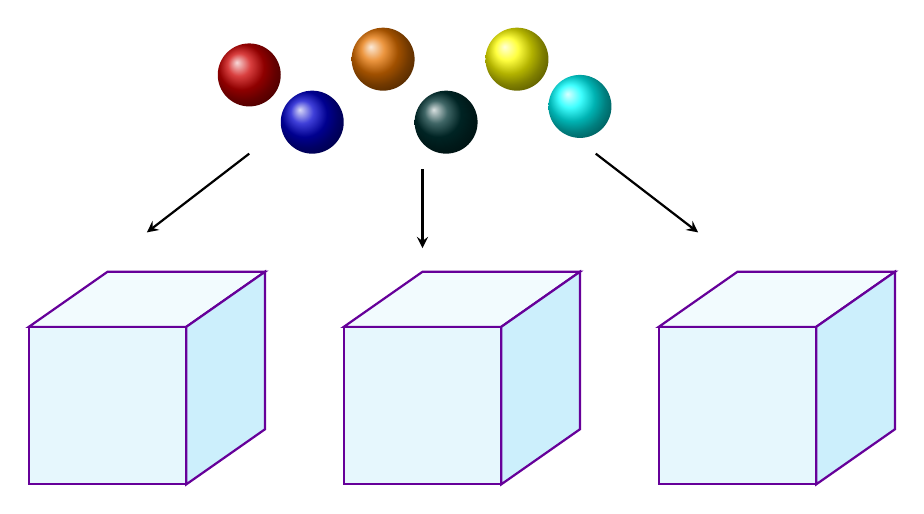
\begin{tikzpicture}[
			cube/.pic={
				\filldraw[fill=cyan!10, draw=blue!60!red, thick] (0,0) rectangle (2,2);
				\filldraw[fill=cyan!5, draw=blue!60!red, thick] (0,2) -- ++(1,0.7) -- ++(2,0) -- (2,2) -- cycle;
				\filldraw[fill=cyan!20, draw=blue!60!red, thick] (2,0) -- (2,2) -- ++(1,0.7) -- ++(0,-2) -- cycle;
			},
			myarrow/.style={->, >=stealth, thick, black},
			ball/.style={circle, draw=none, minimum size=0.8cm}
			]
			\path (0,0) pic {cube};
			\path (4,0) pic {cube};
			\path (8,0) pic {cube};
			\coordinate (topcenter) at (5, 4.5);
			\shade[ball color=red!80!black] (2.8, 5.2) circle (0.4cm); % Đỏ
			\shade[ball color=orange!90!black] (4.5, 5.4) circle (0.4cm); % Cam/Vàng đất
			\shade[ball color=yellow] (6.2, 5.4) circle (0.4cm); % Vàng
			\shade[ball color=blue!80!black] (3.6, 4.6) circle (0.4cm); % Xanh dương đậm
			\shade[ball color=teal!40!black] (5.3, 4.6) circle (0.4cm); % Xanh đen/Teal
			\shade[ball color=cyan] (7.0, 4.8) circle (0.4cm); % Xanh nhạt
			\draw[myarrow] (2.8, 4.2) -- (1.5, 3.2);
			\draw[myarrow] (5.0, 4.0) -- (5.0, 3.0);
			\draw[myarrow] (7.2, 4.2) -- (8.5, 3.2);
		\end{tikzpicture}
	\end{center}
	\loigiai{
		Các trường hợp có thể xảy ra (chú ý thứ tự các hộp không quan trọng).
		\begin{enumerate}
			\item\textbf{Trường hợp 1}. Số viên bi trong ba hộp là $1$, $1$ và $4$.\\
			Chọn $4$ viên bi vào một hộp có $\mathrm{C}_6^4$, hai viên bi còn lại chia vào hai hộp có đúng $1$ cách.\\
			Trường hợp này có tất cả $\mathrm{C}_6^4\cdot 1=15$ cách.
			\item\textbf{Trường hợp 2}. Số viên bi trong ba hộp là $1$, $2$ và $3$.\\
			Chọn $3$ viên bi vào một hộp có $\mathrm{C}_6^3$, ba viên bi còn lại chọn một viên cho vào $1$ hộp có $\mathrm{C}_3^1$ và hai viên cuối cùng bỏ vào hộp còn lại.\\
			Trường hợp này có tất cả $\mathrm{C}_6^3\cdot \mathrm{C}_3^1=60$ cách.
			\item\textbf{Trường hợp 3}. Số viên bi trong ba hộp là $2$, $2$ và $2$.\\
			Bỏ một viên bi nào đó (giả sử là viên bi $A$) vào một hộp có đúng $1$ cách (vì các hộp là như nhau).\\
			Thêm một viên bi vào hộp chứa viên bi $A$ có $5$ cách.\\
			Bốn viên bi còn lại, lấy một viên nào đó (giả sử là viên bi $B$) bỏ vào (một trong) hộp trống có $1$ một cách (vì các hộp là như nhau).\\
			Chọn thêm một viên bi bỏ cùng hộp với $B$ có $3$ cách.\\
			Hai viên bi còn lại thuộc vào hộp cuối cùng.\\
			Trường hợp này có tất cả $1\cdot 5\cdot 1\cdot 3=15$ cách.
		\end{enumerate}
		Vậy có tất cả $15+60+15=90$ cách.\\
		\textit{Chú ý: Trong trường hợp 3 nếu tính bằng cách chọn $2$ viên bi trong $6$ cho vào một hộp, chọn $2$ viên bi trong $4$ viên còn lại cho vào hộp thứ hai, các viên bi còn lại cho vào hộp cuối cùng thì có $\mathrm{C}_6^2\cdot \mathrm{C}_4^2=90$ cách nhưng không xét tính thứ tự của các hộp nên mỗi cách chia sẽ lặp lại $3!=6$ lần.}}
\end{ex}
%%%=============================%%%
\Closesolutionfile{ans}
\newpage
\indapan{12}{ans/ansTN-Dung}
\indapan[TF]{2}{ans/ansTN-DungSai}
\indapan[SA]{6}{ans/ansTN-DienKhuyet}
%%%%%%%%%%%%%%
%%nhãn kết thúc đề (để đếm số trang tự động mỗi đề)
\label{B\thedeso}